% This file was created with tikzplotlib v0.10.1.
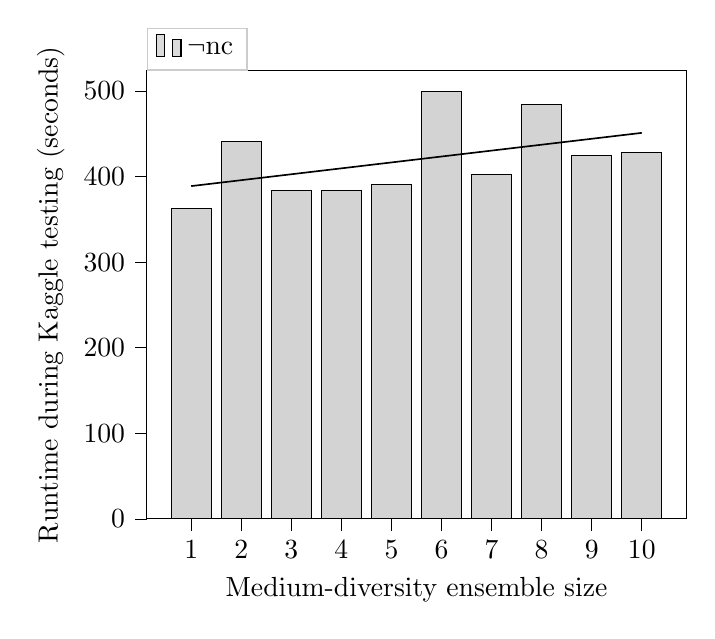
\begin{tikzpicture}

\definecolor{darkgray176}{RGB}{176,176,176}
\definecolor{lightgray}{RGB}{211,211,211}
\definecolor{lightgray204}{RGB}{204,204,204}

\begin{axis}[
legend cell align={left},
legend style={
  fill opacity=0.8,
  draw opacity=1,
  text opacity=1,
  at={(0,1)},
  anchor=south west,
  draw=lightgray204
},
tick align=outside,
tick pos=left,
x grid style={darkgray176},
xlabel={Medium-diversity ensemble size},
xmin=-0.89, xmax=9.89,
xtick style={color=black},
xtick={0,1,2,3,4,5,6,7,8,9},
xticklabels={1,2,3,4,5,6,7,8,9,10},
y grid style={darkgray176},
ylabel={Runtime during Kaggle testing (seconds)},
ymin=0, ymax=523.74,
ytick style={color=black}
]
\draw[draw=black,fill=lightgray] (axis cs:-0.4,0) rectangle (axis cs:0.4,362.7);
\addlegendimage{ybar,ybar legend,draw=black,fill=lightgray}
\addlegendentry{$\neg$nc}

\draw[draw=black,fill=lightgray] (axis cs:0.6,0) rectangle (axis cs:1.4,440.6);
\draw[draw=black,fill=lightgray] (axis cs:1.6,0) rectangle (axis cs:2.4,384);
\draw[draw=black,fill=lightgray] (axis cs:2.6,0) rectangle (axis cs:3.4,383.5);
\draw[draw=black,fill=lightgray] (axis cs:3.6,0) rectangle (axis cs:4.4,390.3);
\draw[draw=black,fill=lightgray] (axis cs:4.6,0) rectangle (axis cs:5.4,498.8);
\draw[draw=black,fill=lightgray] (axis cs:5.6,0) rectangle (axis cs:6.4,402.7);
\draw[draw=black,fill=lightgray] (axis cs:6.6,0) rectangle (axis cs:7.4,483.7);
\draw[draw=black,fill=lightgray] (axis cs:7.6,0) rectangle (axis cs:8.4,424.4);
\draw[draw=black,fill=lightgray] (axis cs:8.6,0) rectangle (axis cs:9.4,428.1);
\addplot [semithick, black, forget plot]
table {%
0 388.794545454545
1 395.702424242424
2 402.610303030303
3 409.518181818182
4 416.42606060606
5 423.333939393939
6 430.241818181818
7 437.149696969697
8 444.057575757576
9 450.965454545454
};
\end{axis}

\end{tikzpicture}
